\chapter{Design}

\section{Planning pivot...}

I plan to change my current strategy in the following ways:

\begin{itemize}
    
 \item Allocate task stacks in the heap. Effectively all protected process mem will be in heap.
 \item Enlarge the heap and allocate more MPU regions to it so it can be further subdivided.
    \begin{itemize}
        \item Supports more processes, increased flexibility.
    \end{itemize}
 \item Support isolating process memory
    \begin{itemize}
        \item Support complete OS SVC interface
        \item Isolate code and data at the process level
        \item Isolate stacks at the thread level
    \end{itemize}
 \item Be less permissive. Change catch-all region 0 to "No Access"
 \item Protect OS code and data

\end{itemize}


\section{Requirements}

For this project, I will guarantee mutual isolation of tasks' stack and heap memory. Stack-allocated variables in one task shall not be readable nor writable by any other task. Similarly, memory allocated to a task on the heap will not be readable nor writable by any other task (until is freed and reallocated). My design will also aim to add minimal overhead to the OS. The MPU hardware should not be massively reconfigured at every context switch.

This implementation supports process loading from disk (introduced in lab 5 of EE380L). Code and data of a loaded process will belong to the process control block and will be accessible to all child tasks. However, the stacks of each task in the process will remain mutually isolated. Also, any heap memory allocated to a task will be accessible only to it -- not to any other task in the system.

Importantly, this implementation does not protect task code if the task is compiled with the OS (i.e. not loaded as a process from disk). Tasks compiled into the OS executable are able to execute any functions that they can be linked against. However, as previously mentioned, code and data of loaded processes \textit{are} protected.

Task memory will be protected automatically upon task creation and heap allocation.

As a proof of concept, my implementation can protect memory of up to twenty-nine different tasks. It cannot scale indefinitely. This is in part due to limitations of the MPU, which imposes a limit on the number of regions that can be individually configured. In a system that must support more tasks, the implementation could be changed to make protecting task memory optional, so that while only sixteen can be protected, more than that may run in the system at any given time.

\section{MPU Functionality}

The MPU is a hardware unit used to protect regions of memory. It supports up to eight configurable memory regions. Each region is configured with a base address, size, and permissions for both privileged and unprivileged access. The region's base address must be aligned to the size of the region. Each region is further divided into eight equally-sized subregions which can be individually enabled or disabled. My design will leverage subregions heavily to maximize the number of tasks that can be mutually isolated.

The MPU implements relative priority between regions. Regions are indexed 0 to 7 where a higher index indicates priority over lower indices. For a given memory access, the MPU region with the highest index containing the relevant address will be used to authorize the access.

\section{Heap Protection}

The heap is implemented as a simple Knuth heap, based upon the implementation from lab 5, with some changes to accomodate the MPU. Any memory allocated to a task on the heap is guaranteed to be isolated from other tasks. This is achieved by grouping memory allocations together into MPU subregions by the owner task. When tasks are allocated memory, the heap manager associates the task's ID with all MPU subregions touched by the allocated block. The task now ``owns'' those subregions, and no other task will be allocated memory in those subregions. In this way, the heap manager guarantees that every subregion will contain blocks belonging to at most one task. When the last allocated block in a given subregion is freed, the owner task relinquishes ownership of the subregion, and the heap manager is free to allocate memory in that subregion to another task. At this point, protecting the heap is as simple as prohibiting access to heap subregions that the running task doesn't ``own''.

A naive solution would be to statically partition the heap into equal-size pieces and allocate one to each task in the system. However, the approach I have chosen ought to scale better to systems where tasks may vary in their demand for heap memory. For example, if only half of all tasks use the heap, then any blocks statically allocated to the other tasks would go unused -- a huge waste. In the case where there are thirty-two tasks in the system (the maximum) and all of them demand heap memory, my solution will allocate each a subregion and converge to the simpler approach.

\begin{figure}[hbtp]
	\centering
	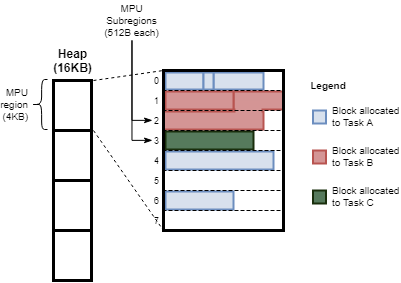
\includegraphics[width=0.7\linewidth]{figs/heap_prot.png}
	\caption{Illustration of how the heap is organized in memory. Four consecutive MPU regions are configured to span the heap, each with eight subregions. Memory allocated to different tasks will always be placed in different subregions such that each subregion's blocks are associated with at most one task. Allocated blocks are shown, color-coded according to which task requested them.}
	\label{fig:heap_prot}
\end{figure}
% https://www.draw.io/#G1K-jvmSFl7cc_w53rWbj7vP-SnMSNnW15

Figure \ref{fig:heap_prot} shows an example heap where three tasks have each been allocated memory. Each subregion will contain memory for at most one task. It's possible for a task's memory to span multiple subregions, as in subregions 1 and 2. This design is susceptible to some amount of internal and external fragmentation, though less than the naive solution I described earlier. You can see internal fragmentation at the end of subregion 0. Only small allocations can fit in the remaining free space of subregion 0, and they must be allocated to Task A to be put there in the first place (since Task A has claimed that subregion). As for external fragmentation, suppose Task C were to request 256 Bytes from the heap manager -- this is larger than one subregion. For that reason, the allocation \textit{could not} fit in the empty subregion 5. It would instead be placed in subregions 7 and 8, leaving subregion 5 to go to waste until a small enough block could be allocated there.

\section{Stack Protection}

To protect tasks' stack memory, I simply allocate stack memory on the heap to the relevant task. This approach is more flexible than a stack pool, where stacks of a certain maximum size must be statically allocated, which can lead to wasted memory.

\section{Fragmentation}

As discussed previously, this design exhibits some amount of internal and external fragmentation.
Here we will discuss the net effect of fragmentation and ways of addressing it.

\subsection{Internal Fragmentation}

The design exhibits internal fragmentation when a task requests more memory than can fit in the remaining free space in a subregion it already owns. The heap manager will go allocate another subregion to the task, or worse, will fail to allocate memory, leaving the hole in the first subregion to go to waste.

This is particularly noticeable in systems that spawn many threads. The OS itself is allocated memory on the heap as needed for TCBs. This memory is protected just like any other heap memory, which means the OS is allocated MPU subregions. Immediately after allocating space for the TCB, space is allocated for the task stack. This means that the OS's MPU subregion will be followed by a task's MPU subregion, since the heap manager allocates subregions sequentially. This means that as the OS fills up its subregion, it is likely to experience internal fragmentation. See Figure \ref{fig:internal_frag} for an illustration of the problem.

\begin{figure}[hbtp]
	\centering
	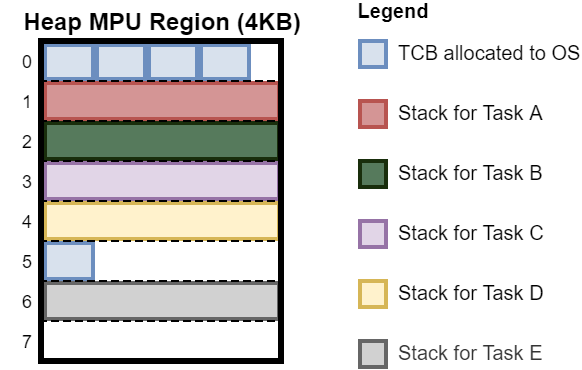
\includegraphics[width=0.7\linewidth]{figs/OS_int_frag.png}
	\caption{Internal fragmentation as experienced by the OS during TCB allocation. OS subregions are not consecutive, meaning that internal fragmentation can occur in many places.}
	\label{fig:internal_frag}
\end{figure}

This can be solved by pre-allocating a pool of TCBs for the OS to pull from at initialization. By allocating all TCBs at once, the programmer will force all OS subregions to be adjacent. This will reduce internal fragmentation since allocated blocks are allowed to span the boundaries between adjacent subregions as long as both belong to the same entity. This requires knowledge of the target application -- specifically, how many tasks it will require.

\subsection{External Fragmentation}

The design exhibits external fragmentation when a task requests more memory than can fit in the free space made up of one or more \textit{free} MPU subregions. This will occur when tasks free all of the memory they own in a given subregion, and the subregion becomes free while its neighboring subregions are still occupied. See Figure \ref{fig:external_frag} for an illustration of the problem.

\begin{figure}[hbtp]
	\centering
	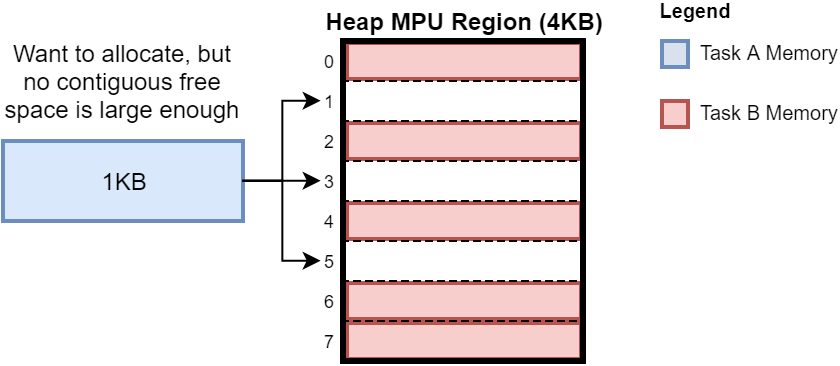
\includegraphics[width=0.7\linewidth]{figs/ext_frag.png}
	\caption{External fragmentation. Though the total amount of free space is larger than the requested block, it cannot fit since there is no \textit{contiguous} region of free space large enough.}
	\label{fig:external_frag}
\end{figure}

\section{Changes to TCB, PCB, and Context Switch}

The TCB and PCB are expanded to include a struct of type \texttt{heap\_owner\_t} used by the heap manager to manage MPU subregions. The TCB now also contains a pointer to the base of its stack, which used to free the task stack upon killing the task. These changes are italicized in Listings \ref{lst:pcb} and \ref{lst:tcb}. The contents of the \texttt{heap\_owner\_t} struct are shown in Listing \ref{lst:heap_owner_t}.
\begin{lstlisting}[language=c, caption={Process Control Block definition}, captionpos=b, label={lst:pcb}, float]
typedef struct _pcb_s
{
    unsigned long num_threads;
    void *text;
    void *data;
    (*@\textit{heap\_owner\_t h\_o;}@*)
} pcb_t;
\end{lstlisting}
\begin{lstlisting}[language=c, caption={Task Control Block definition}, captionpos=b, label={lst:tcb}, float]
typedef struct _tcb_s
{
    long *sp;
    struct _tcb_s *next;
    uint32_t wake_time;
    unsigned long id;
    uint8_t priority;
    uint32_t period;
    unsigned long magic;
    void (*task)(void);
    char * task_name;
    pcb_t *parent_process;
    (*@\textit{long *stack\_base;}@*)
    (*@\textit{heap\_owner\_t h\_o;}@*)
} tcb_t;
\end{lstlisting}
\begin{lstlisting}[language=c, caption={heap\_owner\_t struct definition}, captionpos=b, label={lst:heap_owner_t}, float]
typedef struct _heap_owner_s
{
    unsigned long id;
    uint32_t heap_prot_msk;
} heap_owner_t;
\end{lstlisting}

The \texttt{heap\_owner\_t} struct is a handle used by the heap manager to identify tasks and processes in the system whose memory ought to be mutually isolated. The \texttt{id} field uniquely identifies the memory's owner, whether that be a task or a process. The heap manager will allow blocks with the same owner ID to be grouped together in the same subregion; blocks with different owner IDs must be placed in different subregions. The \texttt{heap\_prot\_msk} field is a mask indicating which heap subregions this task or process has memory in and therefore ought to be allowed to access.

During a context switch, the OS configures the MPU to allow access only to heap subregions associated with the next running task. This is indicated by the \texttt{heap\_prot\_msk} field in the \texttt{heap\_owner\_t} struct of the TCB \textit{and} PCB (if applicable) associated with the next task. All other subregions (either associated with other tasks or unused) are protected. The pseudo-code in Listing \ref{lst:subregions} illustrates this procedure.

\begin{lstlisting}[language=c, caption={Pseudo-code demonstrating how subregions are made accessible based on the TCB \textit{and} PCB.}, captionpos=b, label={lst:subregions}, float]
u32 accessible_subregions = tcb->h_o.heap_prot_msk;

if(tcb->parent_process)
{
  accessible_subregions |= tcb->parent_process->h_o.heap_prot_msk;
}

MPU_ConfigureSubregions(accessible_subregions);

\end{lstlisting}

The MPU regions themselves do not need to be reprogrammed at each context switch. These are programmed once at initialization. Only the subregion masks for each region need to be reprogrammed during the context switch. This keeps the context switch fairly light.

\section{Maximum Number of Tasks}

The 16KB heap contains a total of thirty-two subregions. The maximum number of tasks that can be allocated is twenty-nine, as the OS will consume three subregions allocating TCBs and the rest of the subregions are allocated to the tasks.

\section{Final MPU Region Configuration}

Given the design described, MPU regions are configured as in Figure \ref{table:mpu_cfg}

% Please add the following required packages to your document preamble:
% \usepackage{multirow}
\todo{Update with newest regions}

\begin{table}[H]
    \begin{tabular}{|l|l|l|l|l|l|}
    \hline
    \multirow{2}{*}{\textbf{}} & \multicolumn{1}{c|}{\multirow{2}{*}{\textbf{Base}}} & \multicolumn{1}{c|}{\multirow{2}{*}{\textbf{Size}}} & \multicolumn{2}{c|}{\textbf{Access}}                                                  & \multicolumn{1}{c|}{\multirow{2}{*}{\textbf{Notes}}}                                \\ \cline{4-5}
                               & \multicolumn{1}{c|}{}                               & \multicolumn{1}{c|}{}                               & \multicolumn{1}{c|}{\textbf{Unprivileged}} & \multicolumn{1}{c|}{\textbf{Privileged}} & \multicolumn{1}{c|}{}                                                               \\ \hline
    0                          & 0x00000000                                          & 4GB                                                 & R/W                                        & R/W                                      & \begin{tabular}[c]{@{}l@{}}Allow access\\ if no other\\ region applies\end{tabular} \\ \hline
    1                          &                                                     &                                                     &                                            &                                          &                                                                                     \\ \hline
    2                          &                                                     &                                                     &                                            &                                          &                                                                                     \\ \hline
    3                          &                                                     &                                                     &                                            &                                          &                                                                                     \\ \hline
    4                          & \&Heap                                              & 4KB                                                 & None                                       & None                                     & \begin{tabular}[c]{@{}l@{}}Heap\\ region 0\end{tabular}                             \\ \hline
    5                          & \&Heap + 4KB                                        & 4KB                                                 & None                                       & None                                     & \begin{tabular}[c]{@{}l@{}}Heap\\ region 1\end{tabular}                             \\ \hline
    6                          & \&Heap + 8KB                                        & 4KB                                                 & None                                       & None                                     & \begin{tabular}[c]{@{}l@{}}Heap\\ region 2\end{tabular}                       \\ \hline
    7                          & \&Heap + 12KB                                       & 4KB                                                 & None                                       & None                                     & \begin{tabular}[c]{@{}l@{}}Heap\\ region 3\end{tabular}                       \\ \hline
    \end{tabular}
    \caption{MPU Region Configutation.}
    \label{table:mpu_cfg}
    \end{table}

